%% LaTeX-Beamer template for KIT design
%% by Erik Burger, Christian Hammer
%% title picture by Klaus Krogmann
%%
%% version 2.1
%%
%% mostly compatible to KIT corporate design v2.0
%% http://intranet.kit.edu/gestaltungsrichtlinien.php
%%
%% Problems, bugs and comments to
%% burger@kit.edu
\pdfminorversion=4

\documentclass[18pt]{beamer}

\usepackage[utf8]{inputenc}
\usepackage{listings}
%% SLIDE FORMAT

% use 'beamerthemekit' for standard 4:3 ratio
% for widescreen slides (16:9), use 'beamerthemekitwide'

\usepackage{templates/beamerthemekit}
% \usepackage{templates/beamerthemekitwide}

%% TITLE PICTURE

% if a custom picture is to be used on the title page, copy it into the 'logos'
% directory, in the line below, replace 'mypicture' with the 
% filename (without extension) and uncomment the following line
% (picture proportions: 63 : 20 for standard, 169 : 40 for wide
% *.eps format if you use latex+dvips+ps2pdf, 
% *.jpg/*.png/*.pdf if you use pdflatex)

\titleimage{../Media/background}

%% TITLE LOGO

% for a custom logo on the front page, copy your file into the 'logos'
% directory, insert the filename in the line below and uncomment it

\titlelogo{logo}

% (*.eps format if you use latex+dvips+ps2pdf,
% *.jpg/*.png/*.pdf if you use pdflatex)

%% TikZ INTEGRATION

% use these packages for PCM symbols and UML classes
% \usepackage{templates/tikzkit}
% \usepackage{templates/tikzuml}

\usepackage{hyperref}
\usepackage{color}

% speech bubbles
\usepackage{tikz}
\usetikzlibrary{shapes.callouts}
\usetikzlibrary{arrows,positioning}
\usetikzlibrary{calc}

% rotations
\usepackage{rotating}

% strike through in math mode
\usepackage{cancel}

% for embedded video
\usepackage{multimedia}

% for multiline comments
\usepackage{verbatim} 

% the presentation starts here

\title[Lambda Spiel]{Spass beim Lernen der Lambdakalkülprinzipien}
%\subtitle{Spielend die Denkweise des Programmierens lernen}
\author{PSE 2014/2015}

\institute{Farid Elhaddad |  Florian Fervers | Kai Fieger | 	Robert Hochweiss |	Kay Schmitteckert }
\date{\today}

\beamertemplatenavigationsymbolsempty

\begin{document}

% change the following line to "ngerman" for German style date and logos
\selectlanguage{ngerman}

%title page
\begin{frame}
\titlepage
\end{frame}

%\titlelogo{logo}
%\begin{frame}{Motivation}
%Funktionale Programierung ist
%\begin{itemize}[<+->]

%\item kompakt
%\item frei von Seiteneffekten
%\item unabhängig von Anweisungsreihenfolge

 %$\Rightarrow$   leichter verstänlich
 %$\Rightarrow$    weniger Fehler
 

%\item  Der $\lambda$-Kalkül ist eine Theoritische Grundlage der Funktionale Programierung
%\item  Funktionale Programierung und $\lambda$-Kalkül sind zu Kopleziert
%\end{itemize}  
%\end{frame}
\begin{frame}{Ziel}
\begin{itemize}[<+->]
 \item Der $\lambda$-Kalkül für Informatiknachwuchs im Grunschulalter nahebringen
 \item Kinder lernen beim Spielen besser als im Regulären Unterricht 
 \item Enwickelung eines Spiels , das den kinder Spass macht und grund Prinzipien der  $\lambda$-Kalkül beibringt
 \end{itemize}
\end{frame}

\begin{frame}{Spielelemente}
	\begin{itemize}
	\item Weisses Lamm 
	  
	  
\includegraphics[height=1.cm]{Pictures/lamb_white_wom} \thinspace \thinspace \thinspace \thinspace
			 $\Leftrightarrow$ 
			 \thinspace \thinspace \thinspace \thinspace
			$($
	\item Farbiges Lamm 
	%$\lambda$-Abstraktion
	
			
\includegraphics[height=1.cm]{Pictures/lamb_blue_wm}
			\thinspace \thinspace \thinspace \thinspace
			 $\Leftrightarrow$ 
			 \thinspace \thinspace \thinspace \thinspace
			$\lambda x.$
	\item Edelsteine

			
\includegraphics[height=1.cm]{Pictures/gem_blue}
			\thinspace \thinspace \thinspace \thinspace
			 $\Leftrightarrow$ 
			 \thinspace \thinspace \thinspace \thinspace
			$x$
	\item Lambdaausduck wird durch überainander stehende lämmer representiert 
	\end{itemize}
	
\end{frame}

\begin{frame}{Spiel Regeln}
\begin{itemize}
\item Ein Farbiges Lamm kann das vor ihm Stehende freudschaftkreis verzaubern
\item zum Farbigem Lamm gehören alle unter Ihm Stehende Edelsteine 
\item Das zauberende Lamm verliert seinen Zauberstab und seine Farbe , Dabei vewandeln sich , die von ihm betreuten Edelsteine ,   zum Verzauberten Freundenkreis um . 
\item ein weisses lamm verabschiedet sich vom Spiel wenn direkt unter ihm  genau ein Lamm oder einen Edelstein steht .
\end{itemize}
\end{frame}

\begin{frame}{Reduktionsbeispiel}
	

	

\includegraphics[scale=1,7]{Pictures/lamb_long_blue_wm}\thinspace \thinspace   
 
\includegraphics[scale=0.5]{Pictures/gem_green} \thinspace \thinspace 

\includegraphics[scale=0.5]{Pictures/gem_green}
\thinspace \thinspace \thinspace \thinspace \thinspace \thinspace $\Leftrightarrow$ \thinspace \thinspace \thinspace \thinspace \thinspace \thinspace ($\lambda x. \lambda y. $ x y) z z
\\[0.3cm]


\includegraphics[scale=1,7]{Pictures/lamb_red_wm}
\\[0.3cm]

\includegraphics[scale=0.5]{Pictures/gem_blue}

\includegraphics[scale=0.5]{Pictures/gem_red}
	
	
\end{frame}

\begin{frame}{Reduktionsbeispiel}
	
	
	

\includegraphics[scale=1,7]{Pictures/lamb_long_white_wom}\thinspace \thinspace   

\includegraphics[scale=0.5]{Pictures/gem_green}
\thinspace \thinspace \thinspace \thinspace \thinspace \thinspace $\Leftrightarrow$ \thinspace \thinspace \thinspace \thinspace \thinspace \thinspace (($\lambda y. $ z y)  z)
\\[0.3cm]


\includegraphics[scale=1,7]{Pictures/lamb_red_wm}
\\[0.3cm]

\includegraphics[scale=0.5]{Pictures/gem_green}

\includegraphics[scale=0.5]{Pictures/gem_red}
	
	
	
\end{frame}

\begin{frame}{Reduktionsbeispiel}
	
	
	

\includegraphics[scale=1,7]{Pictures/lamb_red_wm}\thinspace \thinspace   

\includegraphics[scale=0.5]{Pictures/gem_green}
\thinspace \thinspace \thinspace \thinspace \thinspace \thinspace $\Leftrightarrow$ \thinspace \thinspace \thinspace \thinspace \thinspace \thinspace ($\lambda y. $ z y)  z
\\[0.3cm]

\includegraphics[scale=0.5]{Pictures/gem_green}

\includegraphics[scale=0.5]{Pictures/gem_red}
	
	
	
\end{frame}

\begin{frame}{Reduktionsbeispiel}
	

\includegraphics[scale=1,7]{Pictures/lamb_white_wom}\thinspace \thinspace   
\thinspace \thinspace \thinspace \thinspace \thinspace \thinspace $\Leftrightarrow$ \thinspace \thinspace \thinspace \thinspace \thinspace \thinspace ( z y)  
\\[0.3cm]

\includegraphics[scale=0.5]{Pictures/gem_green}

\includegraphics[scale=0.5]{Pictures/gem_red}
\end{frame}


\begin{frame}{Reduktionsbeispiel}


\includegraphics[scale=0.5]{Pictures/gem_green}

\includegraphics[scale=0.5]{Pictures/gem_red}
\thinspace \thinspace \thinspace \thinspace \thinspace \thinspace $\Leftrightarrow$ \thinspace \thinspace \thinspace \thinspace \thinspace \thinspace  z z  
\end{frame}

\begin{frame}{Level}
Das Spiel Hat 2  Levelstypen  : 
\begin{itemize}
\item Eingabe-Bestimmung : Der Spieler muss  ein $\lambda$-Term finden der,nach Anwenden Der Spielregeln, zum vorgegebenen Resultat führt 
\item Ausgabe-Bestimmung : Der Spieler muss , das  nach anwenden der Spielregeln entstehende resultat verraten 
\end{itemize}

\end{frame}

\begin{frame}{Spieler Motivieren}
Damit die Kinder sich nicht langweiln , werden Sie duch Belhnung motiviert länger zu Spielen :
\begin{itemize}[<+->]
\item Jeder Erfolgreicher Level wird mit Coins Belohnt
\item Mit Coins kann der Spieler Hintergründe und Songs kaufen 
\item Es werden versteckte Levels angeboten 
\item Statstiken ermöglichen dem spieler und den Bertreuer einen Einblick auf dem Verlauf zu haben 
\end{itemize}
\end{frame}
\begin{frame}{Szenario}
\begin{itemize}
\item Sprachauswahl
 

\includegraphics[scale=0.5]{../gui/_jpeg/registration1}


\end{itemize}
\end{frame}

\begin{frame}{Szenario}
\begin{itemize}
\item Nameneingabe
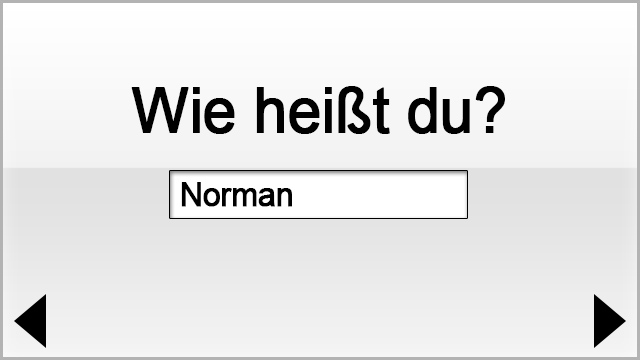
\includegraphics[scale=0.5]{../gui/_jpeg/registration2}
\end{itemize}
\end{frame}

\begin{frame}{Szenario}
\begin{itemize}
\item Awatarauswahl
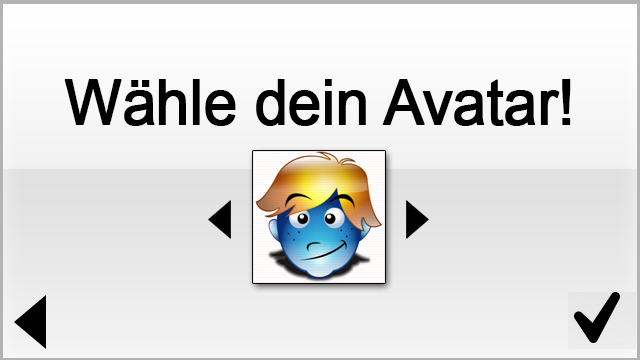
\includegraphics[scale=0.5]{../gui/_jpeg/registration3}
\end{itemize}
\end{frame}

\begin{frame}{Szenario}
\begin{itemize}
\item Wilkommenbildschirm
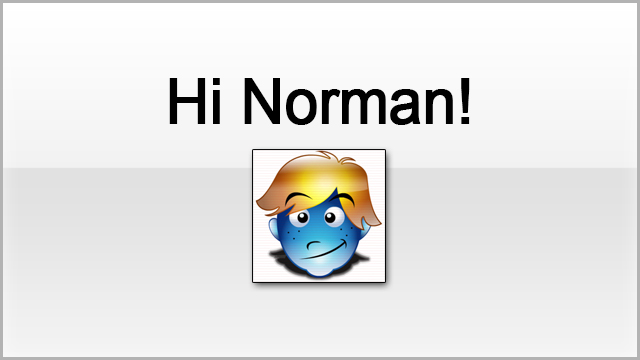
\includegraphics[scale=0.5]{../gui/_jpeg/welcome}
\end{itemize}
\end{frame}

\begin{frame}{Szenario}
\begin{itemize}
\item Hauptmenu
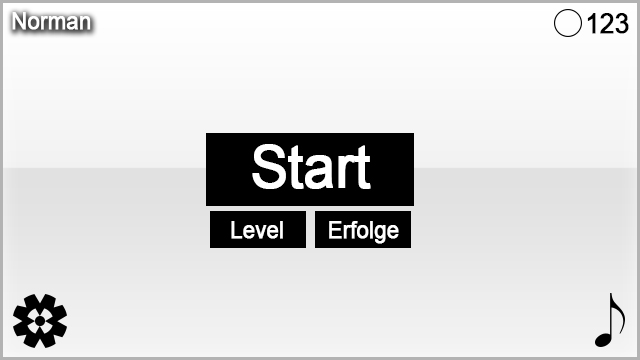
\includegraphics[scale=0.5]{../gui/_jpeg/main_manu}
\end{itemize}
\end{frame}

\begin{frame}{Szenario}
\begin{itemize}
\item Levelmenu
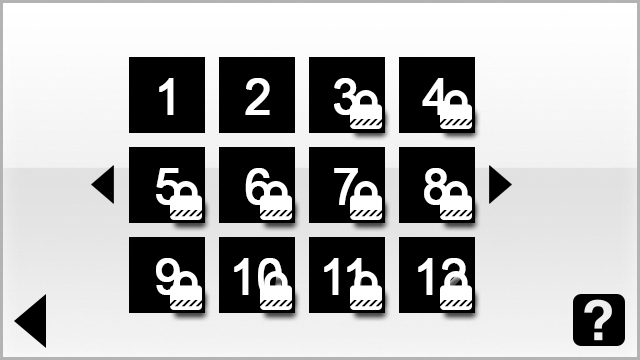
\includegraphics[scale=0.5]{../gui/_jpeg/level}
\end{itemize}
\end{frame}

\begin{frame}{Szenario}
\begin{itemize}
\item Level gestartet 1 
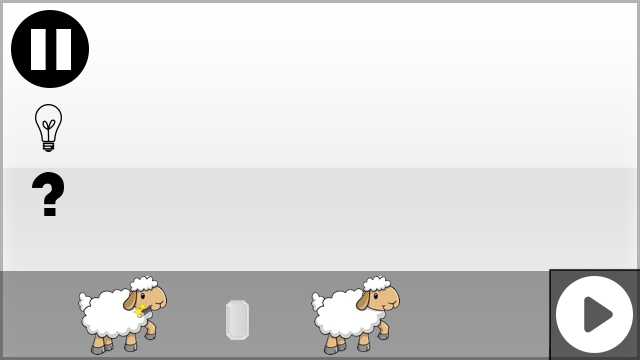
\includegraphics[scale=0.5]{../gui/_jpeg/game_freemode}
\end{itemize}
\end{frame}

\begin{frame}{Szenario}
\begin{itemize}
\item Level gestartet 2
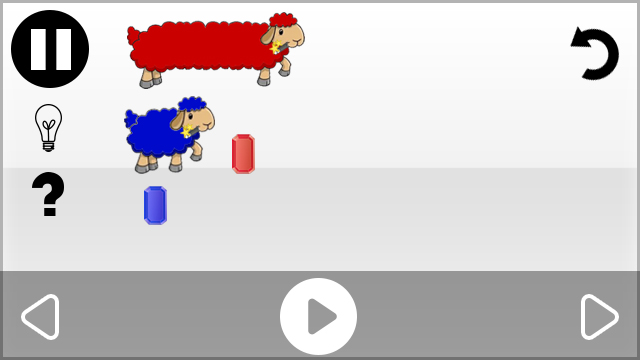
\includegraphics[scale=0.5]{../gui/_jpeg/game_play_started}
\end{itemize}
\end{frame}

\begin{frame}{Szenario}
\begin{itemize}
\item Level gestartet 2
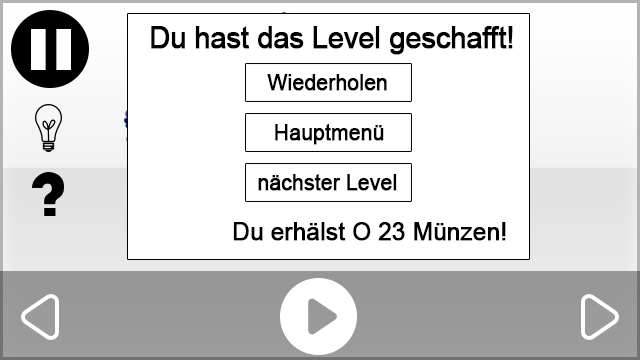
\includegraphics[scale=0.5]{../gui/_jpeg/game_completed}
\end{itemize}
\end{frame}

\begin{frame}
\begin{center}

\color{blue} \Huge Danke fürs Zuhören 
\\[1cm]
\color{blue} \Huge Fragen ??
\end{center}
\end{frame}


\end{document}
